
%% bare_conf.tex
%% V1.3
%% 2007/01/11
%% by Michael Shell
%% See:
%% http://www.michaelshell.org/
%% for current contact information.
%%
%% This is a skeleton file demonstrating the use of IEEEtran.cls
%% (requires IEEEtran.cls version 1.7 or later) with an IEEE conference paper.
%%
%% Support sites:
%% http://www.michaelshell.org/tex/ieeetran/
%% http://www.ctan.org/tex-archive/macros/latex/contrib/IEEEtran/
%% and
%% http://www.ieee.org/

%%*************************************************************************
%% Legal Notice:
%% This code is offered as-is without any warranty either expressed or
%% implied; without even the implied warranty of MERCHANTABILITY or
%% FITNESS FOR A PARTICULAR PURPOSE! 
%% User assumes all risk.
%% In no event shall IEEE or any contributor to this code be liable for
%% any damages or losses, including, but not limited to, incidental,
%% consequential, or any other damages, resulting from the use or misuse
%% of any information contained here.
%%
%% All comments are the opinions of their respective authors and are not
%% necessarily endorsed by the IEEE.
%%
%% This work is distributed under the LaTeX Project Public License (LPPL)
%% ( http://www.latex-project.org/ ) version 1.3, and may be freely used,
%% distributed and modified. A copy of the LPPL, version 1.3, is included
%% in the base LaTeX documentation of all distributions of LaTeX released
%% 2003/12/01 or later.
%% Retain all contribution notices and credits.
%% ** Modified files should be clearly indicated as such, including  **
%% ** renaming them and changing author support contact information. **
%%
%% File list of work: IEEEtran.cls, IEEEtran_HOWTO.pdf, bare_adv.tex,
%%                    bare_conf.tex, bare_jrnl.tex, bare_jrnl_compsoc.tex
%%*************************************************************************

% *** Authors should verify (and, if needed, correct) their LaTeX system  ***
% *** with the testflow diagnostic prior to trusting their LaTeX platform ***
% *** with production work. IEEE's font choices can trigger bugs that do  ***
% *** not appear when using other class files.                            ***
% The testflow support page is at:
% http://www.michaelshell.org/tex/testflow/



% Note that the a4paper option is mainly intended so that authors in
% countries using A4 can easily print to A4 and see how their papers will
% look in print - the typesetting of the document will not typically be
% affected with changes in paper size (but the bottom and side margins will).
% Use the testflow package mentioned above to verify correct handling of
% both paper sizes by the user's LaTeX system.
%
% Also note that the "draftcls" or "draftclsnofoot", not "draft", option
% should be used if it is desired that the figures are to be displayed in
% draft mode.
%
\documentclass[conference]{IEEEtran}
\usepackage{blindtext, graphicx}
% Add the compsoc option for Computer Society conferences.
%
% If IEEEtran.cls has not been installed into the LaTeX system files,
% manually specify the path to it like:
% \documentclass[conference]{../sty/IEEEtran}





% Some very useful LaTeX packages include:
% (uncomment the ones you want to load)


% *** MISC UTILITY PACKAGES ***
%
%\usepackage{ifpdf}
% Heiko Oberdiek's ifpdf.sty is very useful if you need conditional
% compilation based on whether the output is pdf or dvi.
% usage:
% \ifpdf
%   % pdf code
% \else
%   % dvi code
% \fi
% The latest version of ifpdf.sty can be obtained from:
% http://www.ctan.org/tex-archive/macros/latex/contrib/oberdiek/
% Also, note that IEEEtran.cls V1.7 and later provides a builtin
% \ifCLASSINFOpdf conditional that works the same way.
% When switching from latex to pdflatex and vice-versa, the compiler may
% have to be run twice to clear warning/error messages.






% *** CITATION PACKAGES ***
%
%\usepackage{cite}
% cite.sty was written by Donald Arseneau
% V1.6 and later of IEEEtran pre-defines the format of the cite.sty package
% \cite{} output to follow that of IEEE. Loading the cite package will
% result in citation numbers being automatically sorted and properly
% "compressed/ranged". e.g., [1], [9], [2], [7], [5], [6] without using
% cite.sty will become [1], [2], [5]--[7], [9] using cite.sty. cite.sty's
% \cite will automatically add leading space, if needed. Use cite.sty's
% noadjust option (cite.sty V3.8 and later) if you want to turn this off.
% cite.sty is already installed on most LaTeX systems. Be sure and use
% version 4.0 (2003-05-27) and later if using hyperref.sty. cite.sty does
% not currently provide for hyperlinked citations.
% The latest version can be obtained at:
% http://www.ctan.org/tex-archive/macros/latex/contrib/cite/
% The documentation is contained in the cite.sty file itself.






% *** GRAPHICS RELATED PACKAGES ***
%
\ifCLASSINFOpdf
  % \usepackage[pdftex]{graphicx}
  % declare the path(s) where your graphic files are
  % \graphicspath{{../pdf/}{../jpeg/}}
  % and their extensions so you won't have to specify these with
  % every instance of \includegraphics
  % \DeclareGraphicsExtensions{.pdf,.jpeg,.png}
\else
  % or other class option (dvipsone, dvipdf, if not using dvips). graphicx
  % will default to the driver specified in the system graphics.cfg if no
  % driver is specified.
  % \usepackage[dvips]{graphicx}
  % declare the path(s) where your graphic files are
  % \graphicspath{{../eps/}}
  % and their extensions so you won't have to specify these with
  % every instance of \includegraphics
  % \DeclareGraphicsExtensions{.eps}
\fi
% graphicx was written by David Carlisle and Sebastian Rahtz. It is
% required if you want graphics, photos, etc. graphicx.sty is already
% installed on most LaTeX systems. The latest version and documentation can
% be obtained at: 
% http://www.ctan.org/tex-archive/macros/latex/required/graphics/
% Another good source of documentation is "Using Imported Graphics in
% LaTeX2e" by Keith Reckdahl which can be found as epslatex.ps or
% epslatex.pdf at: http://www.ctan.org/tex-archive/info/
%
% latex, and pdflatex in dvi mode, support graphics in encapsulated
% postscript (.eps) format. pdflatex in pdf mode supports graphics
% in .pdf, .jpeg, .png and .mps (metapost) formats. Users should ensure
% that all non-photo figures use a vector format (.eps, .pdf, .mps) and
% not a bitmapped formats (.jpeg, .png). IEEE frowns on bitmapped formats
% which can result in "jaggedy"/blurry rendering of lines and letters as
% well as large increases in file sizes.
%
% You can find documentation about the pdfTeX application at:
% http://www.tug.org/applications/pdftex





% *** MATH PACKAGES ***
%
%\usepackage[cmex10]{amsmath}
% A popular package from the American Mathematical Society that provides
% many useful and powerful commands for dealing with mathematics. If using
% it, be sure to load this package with the cmex10 option to ensure that
% only type 1 fonts will utilized at all point sizes. Without this option,
% it is possible that some math symbols, particularly those within
% footnotes, will be rendered in bitmap form which will result in a
% document that can not be IEEE Xplore compliant!
%
% Also, note that the amsmath package sets \interdisplaylinepenalty to 10000
% thus preventing page breaks from occurring within multiline equations. Use:
%\interdisplaylinepenalty=2500
% after loading amsmath to restore such page breaks as IEEEtran.cls normally
% does. amsmath.sty is already installed on most LaTeX systems. The latest
% version and documentation can be obtained at:
% http://www.ctan.org/tex-archive/macros/latex/required/amslatex/math/





% *** SPECIALIZED LIST PACKAGES ***
%
%\usepackage{algorithmic}
% algorithmic.sty was written by Peter Williams and Rogerio Brito.
% This package provides an algorithmic environment fo describing algorithms.
% You can use the algorithmic environment in-text or within a figure
% environment to provide for a floating algorithm. Do NOT use the algorithm
% floating environment provided by algorithm.sty (by the same authors) or
% algorithm2e.sty (by Christophe Fiorio) as IEEE does not use dedicated
% algorithm float types and packages that provide these will not provide
% correct IEEE style captions. The latest version and documentation of
% algorithmic.sty can be obtained at:
% http://www.ctan.org/tex-archive/macros/latex/contrib/algorithms/
% There is also a support site at:
% http://algorithms.berlios.de/index.html
% Also of interest may be the (relatively newer and more customizable)
% algorithmicx.sty package by Szasz Janos:
% http://www.ctan.org/tex-archive/macros/latex/contrib/algorithmicx/




% *** ALIGNMENT PACKAGES ***
%
%\usepackage{array}
% Frank Mittelbach's and David Carlisle's array.sty patches and improves
% the standard LaTeX2e array and tabular environments to provide better
% appearance and additional user controls. As the default LaTeX2e table
% generation code is lacking to the point of almost being broken with
% respect to the quality of the end results, all users are strongly
% advised to use an enhanced (at the very least that provided by array.sty)
% set of table tools. array.sty is already installed on most systems. The
% latest version and documentation can be obtained at:
% http://www.ctan.org/tex-archive/macros/latex/required/tools/


%\usepackage{mdwmath}
%\usepackage{mdwtab}
% Also highly recommended is Mark Wooding's extremely powerful MDW tools,
% especially mdwmath.sty and mdwtab.sty which are used to format equations
% and tables, respectively. The MDWtools set is already installed on most
% LaTeX systems. The lastest version and documentation is available at:
% http://www.ctan.org/tex-archive/macros/latex/contrib/mdwtools/


% IEEEtran contains the IEEEeqnarray family of commands that can be used to
% generate multiline equations as well as matrices, tables, etc., of high
% quality.


%\usepackage{eqparbox}
% Also of notable interest is Scott Pakin's eqparbox package for creating
% (automatically sized) equal width boxes - aka "natural width parboxes".
% Available at:
% http://www.ctan.org/tex-archive/macros/latex/contrib/eqparbox/





% *** SUBFIGURE PACKAGES ***
%\usepackage[tight,footnotesize]{subfigure}
% subfigure.sty was written by Steven Douglas Cochran. This package makes it
% easy to put subfigures in your figures. e.g., "Figure 1a and 1b". For IEEE
% work, it is a good idea to load it with the tight package option to reduce
% the amount of white space around the subfigures. subfigure.sty is already
% installed on most LaTeX systems. The latest version and documentation can
% be obtained at:
% http://www.ctan.org/tex-archive/obsolete/macros/latex/contrib/subfigure/
% subfigure.sty has been superceeded by subfig.sty.



%\usepackage[caption=false]{caption}
%\usepackage[font=footnotesize]{subfig}
% subfig.sty, also written by Steven Douglas Cochran, is the modern
% replacement for subfigure.sty. However, subfig.sty requires and
% automatically loads Axel Sommerfeldt's caption.sty which will override
% IEEEtran.cls handling of captions and this will result in nonIEEE style
% figure/table captions. To prevent this problem, be sure and preload
% caption.sty with its "caption=false" package option. This is will preserve
% IEEEtran.cls handing of captions. Version 1.3 (2005/06/28) and later 
% (recommended due to many improvements over 1.2) of subfig.sty supports
% the caption=false option directly:
%\usepackage[caption=false,font=footnotesize]{subfig}
%
% The latest version and documentation can be obtained at:
% http://www.ctan.org/tex-archive/macros/latex/contrib/subfig/
% The latest version and documentation of caption.sty can be obtained at:
% http://www.ctan.org/tex-archive/macros/latex/contrib/caption/




% *** FLOAT PACKAGES ***
%
%\usepackage{fixltx2e}
% fixltx2e, the successor to the earlier fix2col.sty, was written by
% Frank Mittelbach and David Carlisle. This package corrects a few problems
% in the LaTeX2e kernel, the most notable of which is that in current
% LaTeX2e releases, the ordering of single and double column floats is not
% guaranteed to be preserved. Thus, an unpatched LaTeX2e can allow a
% single column figure to be placed prior to an earlier double column
% figure. The latest version and documentation can be found at:
% http://www.ctan.org/tex-archive/macros/latex/base/



%\usepackage{stfloats}
% stfloats.sty was written by Sigitas Tolusis. This package gives LaTeX2e
% the ability to do double column floats at the bottom of the page as well
% as the top. (e.g., "\begin{figure*}[!b]" is not normally possible in
% LaTeX2e). It also provides a command:
%\fnbelowfloat
% to enable the placement of footnotes below bottom floats (the standard
% LaTeX2e kernel puts them above bottom floats). This is an invasive package
% which rewrites many portions of the LaTeX2e float routines. It may not work
% with other packages that modify the LaTeX2e float routines. The latest
% version and documentation can be obtained at:
% http://www.ctan.org/tex-archive/macros/latex/contrib/sttools/
% Documentation is contained in the stfloats.sty comments as well as in the
% presfull.pdf file. Do not use the stfloats baselinefloat ability as IEEE
% does not allow \baselineskip to stretch. Authors submitting work to the
% IEEE should note that IEEE rarely uses double column equations and
% that authors should try to avoid such use. Do not be tempted to use the
% cuted.sty or midfloat.sty packages (also by Sigitas Tolusis) as IEEE does
% not format its papers in such ways.





% *** PDF, URL AND HYPERLINK PACKAGES ***
%
\usepackage{url}
% url.sty was written by Donald Arseneau. It provides better support for
% handling and breaking URLs. url.sty is already installed on most LaTeX
% systems. The latest version can be obtained at:
% http://www.ctan.org/tex-archive/macros/latex/contrib/misc/
% Read the url.sty source comments for usage information. Basically,
% \url{my_url_here}.





% *** Do not adjust lengths that control margins, column widths, etc. ***
% *** Do not use packages that alter fonts (such as pslatex).         ***
% There should be no need to do such things with IEEEtran.cls V1.6 and later.
% (Unless specifically asked to do so by the journal or conference you plan
% to submit to, of course. )


% correct bad hyphenation here
\hyphenation{op-tical net-works semi-conduc-tor}


\begin{document}
%
% paper title
% can use linebreaks \\ within to get better formatting as desired
\title{Security in the Internet of Things (IoT)}


% author names and affiliations
% use a multiple column layout for up to three different
% affiliations
\author{\IEEEauthorblockN{Niklas Lensing}
\IEEEauthorblockA{School of Electronic Information and\\Electrical Engineering\\
Shanghai Jiao Tong University\\
Email: Niklas.Lensing@gmail.com}}

% conference papers do not typically use \thanks and this command
% is locked out in conference mode. If really needed, such as for
% the acknowledgment of grants, issue a \IEEEoverridecommandlockouts
% after \documentclass

% for over three affiliations, or if they all won't fit within the width
% of the page, use this alternative format:
% 
%\author{\IEEEauthorblockN{Michael Shell\IEEEauthorrefmark{1},
%Homer Simpson\IEEEauthorrefmark{2},
%James Kirk\IEEEauthorrefmark{3}, 
%Montgomery Scott\IEEEauthorrefmark{3} and
%Eldon Tyrell\IEEEauthorrefmark{4}}
%\IEEEauthorblockA{\IEEEauthorrefmark{1}School of Electrical and Computer Engineering\\
%Georgia Institute of Technology,
%Atlanta, Georgia 30332--0250\\ Email: see http://www.michaelshell.org/contact.html}
%\IEEEauthorblockA{\IEEEauthorrefmark{2}Twentieth Century Fox, Springfield, USA\\
%Email: homer@thesimpsons.com}
%\IEEEauthorblockA{\IEEEauthorrefmark{3}Starfleet Academy, San Francisco, California 96678-2391\\
%Telephone: (800) 555--1212, Fax: (888) 555--1212}
%\IEEEauthorblockA{\IEEEauthorrefmark{4}Tyrell Inc., 123 Replicant Street, Los Angeles, California 90210--4321}}




% use for special paper notices
%\IEEEspecialpapernotice{(Invited Paper)}




% make the title area
\maketitle


\begin{abstract}
%\boldmath
This paper deals with security in the Internet of Things (IoT). 

In a brief introduction it will be elaborated about what the IoT is. 
Subsequently it will be explained why security in the IoT is important with the 
help of some examples. 

The main focus of this paper is the analysis of the current status of security. 
Findings from different organizations are being discussed and then evaluated.

Finally some thoughts about improving the current security situation are 
expressed.

\end{abstract}
% IEEEtran.cls defaults to using nonbold math in the Abstract.
% This preserves the distinction between vectors and scalars. However,
% if the journal you are submitting to favors bold math in the abstract,
% then you can use LaTeX's standard command \boldmath at the very start
% of the abstract to achieve this. Many IEEE journals frown on math
% in the abstract anyway.

% Note that keywords are not normally used for peerreview papers.
\begin{IEEEkeywords}
Internet of Things, IoT, security, security threats.
\end{IEEEkeywords}






% For peer review papers, you can put extra information on the cover
% page as needed:
% \ifCLASSOPTIONpeerreview
% \begin{center} \bfseries EDICS Category: 3-BBND \end{center}
% \fi
%
% For peerreview papers, this IEEEtran command inserts a page break and
% creates the second title. It will be ignored for other modes.
\IEEEpeerreviewmaketitle



\section{Introduction}
The Internet of things (IoT) is a trending topic. Some say that the IoT will 
shape our future lives. But what exactly is this Internet of Things?

The International Telecommunication Union (ITU) states that: ''The Internet of 
Things is the network of physical objects or 'things' embedded with  
electronics, software, sensors, and network connectivity, which 
enables these objects to collect and exchange data.'' \cite{ituPage}

The Oxford University published a definition seeing the IoT as ''a 
proposed development of the Internet in which everyday objects have network 
connectivity, allowing them to send and receive data.'' \cite{HPstudy}

Furthermore HP observes that ''suddenly, everything from refrigerators to 
sprinkler systems are wired and interconnected (...). These devices are now 
collectively called the Internet of Things (IoT).'' \cite{HPstudy}

As one can see from these three citations there is no fixed definition of what 
the Internet of Things is. Bringing the key points together one can learn that 
they all stress the idea of devices being connected to the Internet to exchange 
information. This is a quite spacious definition allowing lots of devices to 
count themselves into the range of IoT devices.

Another point that can be observed is the diversity of the entities being 
involved into the IoT. These three quotes are from an international 
standardization organization, a famous university and a big IT company. So it 
can be concluded that there are different stakeholders being involved into the 
IoT. It is a topic which affects several areas and therefore attracts so many 
different entities.

Due to the growing importance of IoT and it's seemingly endless possibilities 
it naturally also attracts the attention of hackers. As a consequence one might 
ask: What is done about security in the IoT? Do we actually need it all? These 
are the questions that this paper will focus on.


\section{Why is security in the IoT important?}
Not securing your IoT devices properly can have serious consequences. Hacked 
IoT devices can be very dangerous in the hands of people with bad intentions. 
They could either manipulate the device so that it causes damage to others or 
steal the information stored on this device. 

What is more the IoT is becoming more and more interesting for hackers as it is 
growing fast and a lot of money is involved. Both factors that make it a 
lucrative target. 

\subsection{Hacked ''things'' can lead to serious problems - an example}
A popular example for emphasizing that security in the IoT is very important is 
a security flaw in the Jeep Cherokee. The Jeep Cherokee is an all-terrain 
vehicle which features an infotainment system called UConnect. The US model 
features a modem which connects the car to the Internet. With the help of this 
modem hackers were able to hack over the Internet into UConnect which in turn 
had access to the car's central CAN bus system. This CAN bus can be found in a 
lot of modern cars and it is used to distribute information between the car's 
electronic devices. With access to the CAN bus the hackers were able to send 
instructions to the car's brakes, the gas and in reverse gear even to the 
wheel. \cite{ctArticle}

One might ask how it is possible that the infotainment system was entitled to 
do so? Why was there no protection against such non authorized commands?

First of all it has to be stated that connecting the infotainment system to 
other electronic devices in a car is very useful. For instance the 
infotainment system of the Jeep Cherokee adjusts the volume of the music 
according to the speed of the car and to do so it needs to be connected to the 
CAN bus. However the CAN bus was not designed to be secure against hacker 
attacks. When the CAN bus was designed it was a closed system and attacks from 
outside were not an issue. It was not foreseeable that cars would get connected 
to the Internet.

This example shows one of the major problems of IoT devices. A lot of the 
''things'' that are getting connected to the internet now were never designed 
to be secured against hacker attacks. As they were initially not designed to be 
secure, it is very hard to implement security afterwards.

\subsection{Sensitive data processed by ''things'' should be protected}
IoT devices help us in our everyday life. To do so, several of these 
devices have access to very sensitive personal data. 

One example is the Apple Watch which gathers several sensitive information. The 
watch has an integrated heart beat scanner so it holds information about the 
user's health condition. What is more it can be used with Apple's payment 
system Apple Pay and therefore has access to banking information. With the help 
of an IPhone it can also obtain the current GPS position. 

To sum it up an Apple Watch is able to hold information about one's health 
condition, banking and location data. All of these are data which 
surely a lot of people would like to be kept secret. And to keep these data 
secret proper security is necessary.

\subsection{IoTs importance is growing fast}
The IoT is currently a big trend. Researchers, organizations and companies 
engage themselves with the IoT and as a result it is growing fast. According to 
Gartner, by 2020 the IoT will include 26 billion units and it will generate 
incremental revenue exceeding \$300 billion. \cite{gartnerPage}

These figures make it a very lucrative target for hackers. 26 billion units is 
a huge playground that can be hacked and hackers will even be more motivated as 
there is a lot of money involved. Hackers have already proven to be able to 
hack into IoT devices and they will continue to try. As a consequence IoT 
devices should be secured properly.

\section{Current status of security in IoT}
Regarding the arguments and examples from the previous section, security should 
be handled seriously in the IoT. In this section the current status of security 
in IoT will be elaborated. 

To get an overview about the current status a study on security in IoT devices 
and the OWASP Top 10 list will be evaluated. 

What is more it is discussed how IoT devices are being patched.

\subsection{IoT security study}
A current study (\cite{HPstudy}) conducted by Hewlett Packard (HP) evaluated on 
the security of IoT devices. In this study HP searched for security issues in 
IoT devices. They tested 10 IoT devices for common security flaws. These 10 
devices were:

\begin{itemize}
\item TV
\item web cam
\item home thermostat
\item remote power outlet
\item sprinkler controller
\item hub for controlling multiple devices
\item door lock
\item home alarm
\item scale
\item garage door opener
\end{itemize}

Some of these devices have access to sensitive information about the user. The 
TV for example could tell a hacker which programs the user likes to watch. 
Spying on a web cam might gives hackers a very intimate insight into the user's 
life.

Others of these devices are a lucrative target to be manipulated by an 
attacker. A hacked home alarm and door lock would for example facilitate a 
house robbery. 

As a consequence one might anticipate that these devices were secured properly 
against attacks. However the HP study results show different facts.

HP found out that 7 of these 10 devices did not encrypt their network services. 
That means all the information being sent from and to these devices could easily
be intercepted and read by an attacker. 

Furthermore 6 of the devices had insecure web interfaces. HP found security 
loopholes in these web interfaces which allowed them to hack into the device. 
Hackers could have used these loopholes to get access to the device's controls 
without having the permission to do so. 

Several devices also lacked a sufficient password policy: 8 of the devices 
allowed the user to set passwords like ''123'' or ''abc''. A hacker would 
have no problems to find out these passwords and get access to the device.

Finally 7 of the 10 devices allowed attackers to identify valid accounts 
through account enumeration. This means that these devices would tell an 
attacker whether a certain account exists or not. This can be misused to find 
a valid user account and then perform a directed attack on this account. 

Figure \ref{HPStudyresults} shows a summary of all the results from the HP 
study.

\begin{figure}[!t]
\centering
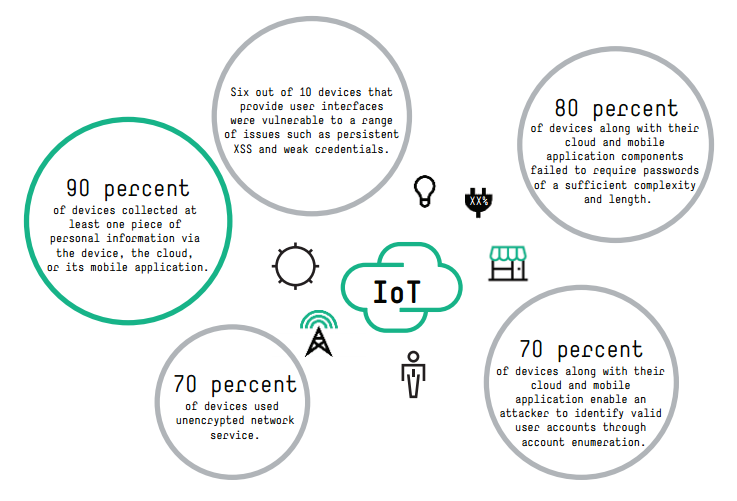
\includegraphics[width=3.5in]{./img/hpStudy1.png}
\caption{HP study results}
\label{HPStudyresults}
\end{figure}

Although these results are concerning one might argue that a study on 10 
devices is not representative for the whole IoT business. It could not be 
proven that these concerning flaws were common in IoT devices. To contradict 
this argument HP argues in \cite[p. 6]{HPstudy}: ''While there are certainly 
large numbers of IoT devices already on the market, and that number continues 
to grow on a daily basis, we believe the similarity in results of this subset 
provides a good indicator of where the market currently stands as it relates to 
security and the internet of things.'' 

Even if this study might not be representative for the whole IoT business: Many 
of the security flaws found by the study are simple flaws. They would not need 
much work to be fixed. So it seems there is either a lack of time or will to 
handle security in at least some IoT business areas.

\subsection{OWASP Top 10}
The Open Web Application Security Project (OWASP) is a foundation which tries 
to enforce security throughout the Internet. To do so, it runs several projects 
which aim to establish a safer Internet. 

Among these projects OWASP publishes a list of the top 10 security flaws in the 
IoT. It lists the most common mistakes done about security ordered by their 
frequency of occurrence. The list can be seen in figure \ref{owaspTop10}. 

\begin{figure}[!t]
\centering
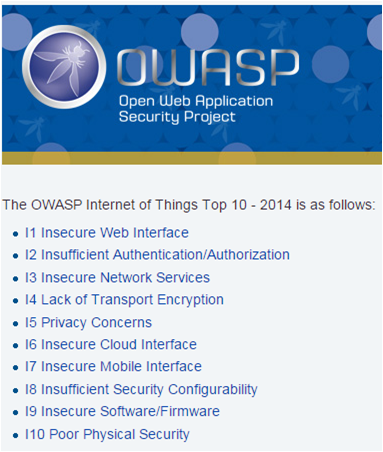
\includegraphics[width=3.0in]{./img/owaspTop10.png}
\caption{The OWASP Internet of Things Top 10}
\label{owaspTop10}
\end{figure}

With this list OWASP wants to give developers an overview about which security 
issues are common and how they should be handled. To every of the 10 security 
flaws exists a detailed page which gives further information on how to take 
counter measures against the threat. Developers who are unfamiliar with  
security topics are supposed to use this page as an information source to 
secure their software properly.

Point 1, 4 and 8 on the Top 10 list were also mentioned in the study which 
was discussed in the previous section: Similar to the points on the Top 10 list 
the HP study found out that many of the devices tested had an insecure web 
interface, did not encrypt their network traffic and featured insufficient 
security configurability which means amongst other things that a sufficient 
password policy is missing. That these points are also mentioned in this Top 
10 list is another indicator that the results of the study are accurate.

According to the top 10 list insufficient authentication/authorization is a 
common security flaw in IoT devices. This flaw comprises bad or non existing 
password encryption and the lack of user roles. 

Passwords should always be encrypted. This includes both, when they are saved 
in a database as well as when they are sent over the network. If this is not 
done a hacker could easily extract the password from network traffic or try to 
steal the database and get the password from there without any effort. 

User roles are essential to a securely working environment. Not all user 
accounts for a system should have the same rights. There should be a 
distinction between different roles. Otherwise every user could change 
passwords or delete users which facilitates the work for attackers.

The third point on the list, insecure network services, is referring to open 
ports on network devices which could be closed as they are not needed. Hackers 
often look for well known ports which are known to offer insecure network 
services. To minimize the risk of being attacked all ports which are not 
absolutely necessary for proper operation should be closed.

Another point mentioned on the list are privacy concerns. When collecting user 
data it should be carefully determined which information are absolutely 
necessary to be stored. User data which is not needed should be discarded to 
make a theft have less impact on the user's privacy. In addition to that it 
should also be clearly determined who is allowed access to sensitive user data. 
Only persons who really need access to the data should get it.

Point 9 and 10 on the Top 10 list are topics which demand a rather high effort 
to be met.

Insecure software/firmware refers to security holes in software. OWASP states 
that there should be a mechanism to update software on IoT devices. As the 
devices are exposed to the Internet hackers will eventually find security holes 
in the software and exploit these holes. Hence there has to be a mechanism to 
fix them.

The last point on the list, poor physical security, states that the devices 
should be stored in a secured place where attackers cannot easily get access 
to. This minimizes the risk of direct physical intervention on the device by an 
attacker.

Analysing the points on the Top 10 list, one can see that the upper points on 
the list are simple security flaws which can be met with rather little effort. 
The more complex and expensive security issues such as an update mechanism or 
ensuring physical security are the last points on the list. Taking into account 
that the points are ordered by their frequency of occurrence it can be 
concluded that not a lot of effort is put into ensuring security in IoT. This 
reflects the findings of the HP study mentioned above which also stated similar 
facts.


\subsection{Patching problems}
Security updates are an important means to fix holes that were not known when a 
software got released. For software which has been exposed to the web for a 
longer time such as operating systems and browsers it is common practice to 
release security patches at least once a month. These patches are then 
distributed over the Internet.

The software update process in IoT is still an unsolved problem in a lot of 
cases. The problem in IoT is that a lot of the devices where the software runs 
on are difficult to update or were not initially designed to get software 
updates. 

One example are cars. For software updates cars normally need to be send back 
to the car manufacturer as only he has the know how to perform software 
updates. However, implementing the practice of sending the car back to the car 
manufacturer every month for security updates is for obvious reasons not 
possible. A different approach is needed.

Another aspect is that several IoT devices are being used a longer time than 
common devices that are connected to the Internet nowadays. As technology is 
developing fast, it is hard to maintain security and interoperability for old 
devices with other, newer web devices. In \cite{arstechnicaPage} one example of 
this problem is given: ''We have one customer monitoring HVAC systems chilling 
a data center, and these industrial chillers last a long time - some are 80 
years old. But the technology for monitoring has a much faster upgrade cycle. 
How do you build an architecture for things like that that's enabled for  
upgradability?'' 

These unsolved patching problems are still unsolved in many business areas of 
the IoT. 


% needed in second column of first page if using \IEEEpubid
%\IEEEpubidadjcol

% An example of a floating figure using the graphicx package.
% Note that \label must occur AFTER (or within) \caption.
% For figures, \caption should occur after the \includegraphics.
% Note that IEEEtran v1.7 and later has special internal code that
% is designed to preserve the operation of \label within \caption
% even when the captionsoff option is in effect. However, because
% of issues like this, it may be the safest practice to put all your
% \label just after \caption rather than within \caption{}.
%
% Reminder: the "draftcls" or "draftclsnofoot", not "draft", class
% option should be used if it is desired that the figures are to be
% displayed while in draft mode.
%
%\begin{figure}[!t]
%\centering
%\includegraphics[width=2.5in]{myfigure}
% where an .eps filename suffix will be assumed under latex, 
% and a .pdf suffix will be assumed for pdflatex; or what has been declared
% via \DeclareGraphicsExtensions.
%\caption{Simulation Results}
%\label{fig_sim}
%\end{figure}

% Note that IEEE typically puts floats only at the top, even when this
% results in a large percentage of a column being occupied by floats.


% An example of a double column floating figure using two subfigures.
% (The subfig.sty package must be loaded for this to work.)
% The subfigure \label commands are set within each subfloat command, the
% \label for the overall figure must come after \caption.
% \hfil must be used as a separator to get equal spacing.
% The subfigure.sty package works much the same way, except \subfigure is
% used instead of \subfloat.
%
%\begin{figure*}[!t]
%\centerline{\subfloat[Case I]\includegraphics[width=2.5in]{subfigcase1}%
%\label{fig_first_case}}
%\hfil
%\subfloat[Case II]{\includegraphics[width=2.5in]{subfigcase2}%
%\label{fig_second_case}}}
%\caption{Simulation results}
%\label{fig_sim}
%\end{figure*}
%
% Note that often IEEE papers with subfigures do not employ subfigure
% captions (using the optional argument to \subfloat), but instead will
% reference/describe all of them (a), (b), etc., within the main caption.


% An example of a floating table. Note that, for IEEE style tables, the 
% \caption command should come BEFORE the table. Table text will default to
% \footnotesize as IEEE normally uses this smaller font for tables.
% The \label must come after \caption as always.
%
%\begin{table}[!t]
%% increase table row spacing, adjust to taste
%\renewcommand{\arraystretch}{1.3}
% if using array.sty, it might be a good idea to tweak the value of
% \extrarowheight as needed to properly center the text within the cells
%\caption{An Example of a Table}
%\label{table_example}
%\centering
%% Some packages, such as MDW tools, offer better commands for making tables
%% than the plain LaTeX2e tabular which is used here.
%\begin{tabular}{|c||c|}
%\hline
%One & Two\\
%\hline
%Three & Four\\
%\hline
%\end{tabular}
%\end{table}


% Note that IEEE does not put floats in the very first column - or typically
% anywhere on the first page for that matter. Also, in-text middle ("here")
% positioning is not used. Most IEEE journals use top floats exclusively.
% Note that, LaTeX2e, unlike IEEE journals, places footnotes above bottom
% floats. This can be corrected via the \fnbelowfloat command of the
% stfloats package.



\section{Conclusion}
It can be stated that currently there is a lack of experience and/or will to 
deal with security properly. Developers seem to invest their time rather into 
new features than into security. This is reflected by the results of the HP 
study and the OWASP Top 10 list. Also the unsolved problem of developing an 
update mechanism shows that there is little motivation to deal with security 
related topics.

No matter where this lack of motivation comes from - no experience or no will - 
security in IoT should and can be dealt with.

Assuming that there is a lack of experience there are means to get information 
such as the OWASP Top 10 list which gives a good introduction into the topic. 
Developers could use the information from this project to secure their IoT 
devices against the most common threats with little effort.

Developers might argue that right now they do not want to deal with security 
and rather prefer to focus on implementing new features. Security could be 
dealt with later. However this way of thinking has proven to be wrong: The 
problems with the CAN bus in the Jeep Cherokee show that implementing security 
after the design can be difficult or even impossible.

As a result security has to be considered in the design of IoT devices. 
Implementing security later is complicated and costs a lot more or is even 
infeasible. It is cheaper - time and money wise - to implement security now. 

One might also ask if really all these ''things'' being connected to the 
Internet right now, do need this connection. Does for instance an iron need an 
Internet connection? There are some which do have one. Perhaps part of the 
solution for the IoT security issues is quite simple: Just do not connect some 
''things'' to the Internet at all. A proper thought about the benefits of 
connecting a device to the Internet might help to reduce security issues.

The aim of this paper is not to condemn the IoT or to make it look as a bad 
idea. This paper just wants to emphasize that security should be considered 
more carefully in the design of IoT devices. The IoT bears a lot of fascinating 
opportunities but while exploring these, security issues should be considered 
and included into the design. Ignoring security threats can lead to severe 
problems as this paper pointed out.


% if have a single appendix:
%\appendix[Proof of the Zonklar Equations]
% or
%\appendix  % for no appendix heading
% do not use \section anymore after \appendix, only \section*
% is possibly needed

% use appendices with more than one appendix
% then use \section to start each appendix
% you must declare a \section before using any
% \subsection or using \label (\appendices by itself
% starts a section numbered zero.)
%


%\appendices
%\section{Proof of the First Zonklar Equation}
%\blindtext
%
%% use section* for acknowledgement
%\section*{Acknowledgment}


%The authors would like to thank...


% Can use something like this to put references on a page
% by themselves when using endfloat and the captionsoff option.
\ifCLASSOPTIONcaptionsoff
  \newpage
\fi



% trigger a \newpage just before the given reference
% number - used to balance the columns on the last page
% adjust value as needed - may need to be readjusted if
% the document is modified later
%\IEEEtriggeratref{8}
% The "triggered" command can be changed if desired:
%\IEEEtriggercmd{\enlargethispage{-5in}}

% references section

% can use a bibliography generated by BibTeX as a .bbl file
% BibTeX documentation can be easily obtained at:
% http://www.ctan.org/tex-archive/biblio/bibtex/contrib/doc/
% The IEEEtran BibTeX style support page is at:
% http://www.michaelshell.org/tex/ieeetran/bibtex/
%\bibliographystyle{IEEEtran}
% argument is your BibTeX string definitions and bibliography database(s)
%\bibliography{IEEEabrv,../bib/paper}
%
% <OR> manually copy in the resultant .bbl file
% set second argument of \begin to the number of references
% (used to reserve space for the reference number labels box)
\begin{thebibliography}{1}

%\bibitem{IEEEhowto:kopka}
%H.~Kopka and P.~W. Daly, \emph{A Guide to \LaTeX}, 3rd~ed.\hskip 1em plus
%  0.5em minus 0.4em\relax Harlow, England: Addison-Wesley, 1999.

\bibitem{ituPage}
International Telecommunication Union (ITU), \emph{Internet of Things Global 
Standards Initiative}, \hskip 1em plus 0.5em minus 0.4em\relax 
\url{http://www.itu.int/en/ITU-T/gsi/iot/Pages/default.aspx}, last access: 
2015-11-03.

\bibitem{owaspPage}
Open Web Application Security Project (OWASP), \emph{OWASP Internet of Things 
Top Ten Project}, \hskip 1em plus 0.5em minus 0.4em\relax 
\url{https://www.owasp.org/index.php/OWASP_Internet_of_Things_Top_Ten_Project#tab=OWASP_Internet_of_Things_Top_10_for_2014},
 last access: 2015-11-03.

\bibitem{HPstudy}
Hewlett Packard (HP), \emph{Internet of things research study}, \hskip 1em plus 
0.5em minus 0.4em\relax  
\url{http://www8.hp.com/h20195/V2/GetPDF.aspx/4AA5-4759ENW.pdf}, last access: 
2015-11-03.

\bibitem{ctArticle}
B.~Benz and F.~A. Scherschel, \emph{Der Feind im Innern}\hskip 1em plus 0.5em 
minus 0.4em\relax c't - Magazin fuer Computer und Technik, Germany: Heise 
Verlag, 21/15.

\bibitem{gartnerPage}
Gartner, \emph{Gartner Says the Internet of Things Installed Base Will Grow to 
26 Billion Units By 2020}, \hskip 1em plus 0.5em minus 0.4em\relax  
\url{http://www.gartner.com/newsroom/id/2636073}, last access: 2015-11-08.

\bibitem{arstechnicaPage}
arstechnica, \emph{The future is the Internet of Things—deal with it}, \hskip 
1em plus 0.5em minus 0.4em\relax  
\url{http://arstechnica.com/unite/2015/10/the-future-is-the-internet-of-things-deal-with-it/},
 last access: 2015-11-10.

\end{thebibliography}

% biography section
% 
% If you have an EPS/PDF photo (graphicx package needed) extra braces are
% needed around the contents of the optional argument to biography to prevent
% the LaTeX parser from getting confused when it sees the complicated
% \includegraphics command within an optional argument. (You could create
% your own custom macro containing the \includegraphics command to make things
% simpler here.)
%\begin{biography}[{\includegraphics[width=1in,height=1.25in,clip,keepaspectratio]{mshell}}]{Michael Shell}
% or if you just want to reserve a space for a photo:

\begin{IEEEbiography}[{\includegraphics[width=1in,height=1.25in,clip,keepaspectratio]{picture}}]{John Doe}
\blindtext
\end{IEEEbiography}

% You can push biographies down or up by placing
% a \vfill before or after them. The appropriate
% use of \vfill depends on what kind of text is
% on the last page and whether or not the columns
% are being equalized.

%\vfill

% Can be used to pull up biographies so that the bottom of the last one
% is flush with the other column.
%\enlargethispage{-5in}




% that's all folks
\end{document}



